\renewcommand{\theequation}{\theenumi}
\begin{enumerate}[label=\arabic*.,ref=\thesubsection.\theenumi]
\numberwithin{equation}{enumi}

\item given $\implies$
\\
\begin{align}
\vec A = \myvec{0\\490}
\\
\vec a = \myvec{0\\-9.8}
\\
\vec v_A = \myvec{1.5\\0}
\\
\vec v_B =  \vec v_A  + \vec a t
\\
\vec d = \vec v_A t + \frac{1}{2}\vec a t^2
\\
\vec B = \vec A + \vec d
\end{align}
\begin{align}
\vec B = \myvec{0\\490} + \myvec{1.5\\0}t +\frac{1}{2}\myvec{0\\-9.8} t^2
\\
\myvec {x\\0} = \myvec{0\\490} + \myvec{1.5\\0}t +\frac{1}{2}\myvec{0\\-9.8} t^2
\\
490 = \frac{1}{2} 9.8t^2
\\
t = 10
\\
\vec v_B = \myvec{1.5\\0} + \myvec{0\\9.8}10 = \myvec{1.5\\98}
\end{align}
\begin{figure}[!ht]
	\centering
	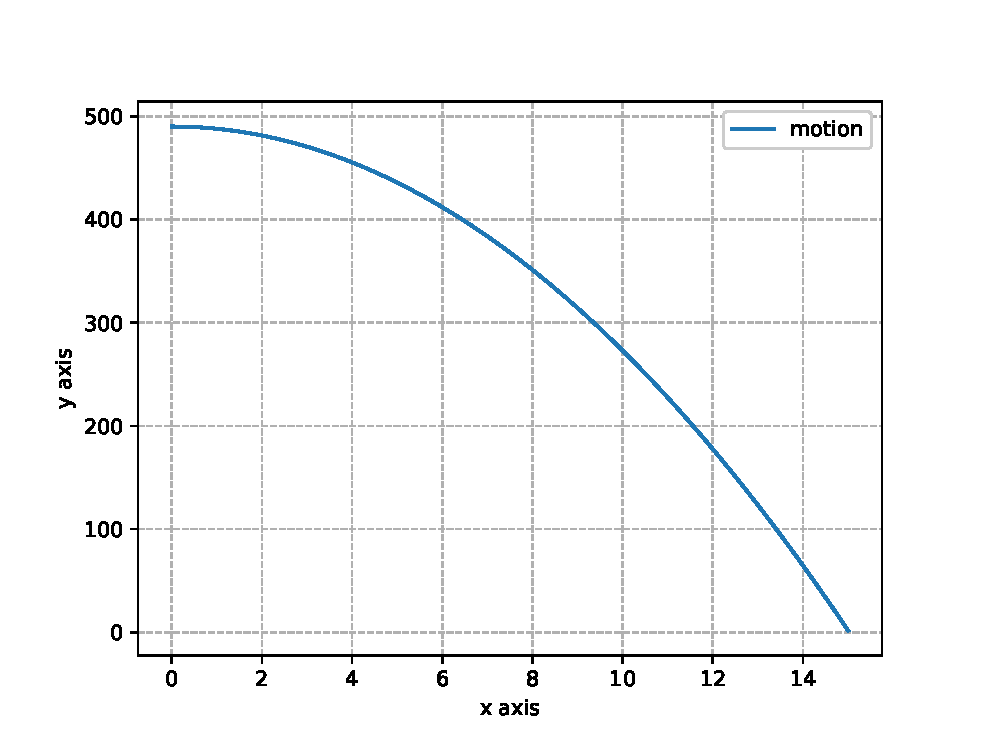
\includegraphics[width=\columnwidth]{./figures/line/motion/motion.eps}
	\caption{motion }
	\label{fig:motion}
\end{figure}

\begin{lstlisting}
codes/line/motion/motion.py
\end{lstlisting}

\end{enumerate}